\chapter{Numerical treatment}
\label{chap:num}
% * numerical treatments necessary
% * main goal: calculate reduced density operator
% * other things: absorption spectra, single trajectories


%%%%%%%%%%%%%%%%%%%%%%%%%%%%%%%%%%%%%%%%%%%%%%%%%%%%%%%%%%%%%%%%%%%%%%%%%%%%%%%
\section{Hierarchical Equations of Motion}
\label{sec:num.heom}
% * Tanimura HEOMs
%%%%%%%%%%%%%%%%%%%%%%%%%%%%%%%%%%%%%%%%%%%%%%%%%%%%%%%%%%%%%%%%%%%%%%%%%%%%%%%


%%%%%%%%%%%%%%%%%%%%%%%%%%%%%%%%%%%%%%%%%%%%%%%%%%%%%%%%%%%%%%%%%%%%%%%%%%%%%%%
\section{Stochastic Hierarchical Equations of Motion}
\label{sec:num.sheom}
% * main idea
%
% TODO more general cases?
%%%%%%%%%%%%%%%%%%%%%%%%%%%%%%%%%%%%%%%%%%%%%%%%%%%%%%%%%%%%%%%%%%%%%%%%%%%%%%%

In this section we present the main results of this work, namely an approach to solve the non-Markovian stochastic Schrödinger equation
\begin{equation}
  \partial \psi_t = -\ii h \psi_t + L\ZZ_t \psi_t - \adj{L}\int_0^t \alpha(t-s) \frac{\delta\psi_t}{\delta\ZZ_s} \dd s
  \label{eq:num.nmsse}
\end{equation}
numerically without resorting to the $O$-operator substitution.
% FIXME Citations
Therefore we need to conceive a different way to deal with the functional derivate's non-locality in time and process realization, as it prevents the application of efficient Monte-Carlo methods, which are used to deal with stochastic Schrödinger equations in the Markovian regime \cite{}.

It turns out that for certain correlation functions the linear \NMSSE~\ref{eq:num.nmsse} is formally equivalent to an infinite hierarchy of completely local stochastic differential equations.
% TODO Really?
Although we borrow the main idea from the hierarchical equations of motion presented in the previous section, we need to deal with some peculiarities of our \NMSSE first.

%%%%%%%%%%%%%%%%%%%%%%%%%%%%%%%%%%%%%%%%%%%%%%%%%%%%%%%%%%%%%%%%%%%%%%%%%%%%%%%
\subsection{Linear Hierarchy}
\label{sub:num.sheom.lin}
% * derivation
% * terminator
%
% TODO Surpession by γ / Ω; differences, in the following combined into w
% TODO Time-local/nonlocal terminators

The basic idea is to absorb the action of the functional derivative on $\psitZ$ into an auxiliary pure state
\begin{equation}
  \psitZ[1] := \int_0^t \alpha(t - s) \frac{\delta \psi_t(\ZZ)}{\delta \ZZ_s} \dd s.
  \label{eq:num.first_order}
\end{equation}
Hereinafter, we use the term \quotes{state} quite loosely for any vector in the system's Hilbert space regardless of its norm.
Recall that the integral boundaries arise only after we apply the derivative on states $\psi_t(\ZZ)$ that satisfy the additional condition $\delta \psitZ / \delta \ZZ_s = 0$ for $ s < 0$ and $s > t$.
Therefore we may write \autoref{eq:num.first_order} more concise as
\begin{equation*}
  \psitZ[1] = \left( \int \alpha(t - s) \frac{\delta}{\delta \ZZ_s} \dd s \right) \psitZ =: \adjZZ_t \psitZ
\end{equation*}
with the integrated functional derivation operator $\adjZZ_t$.
For a finite environment $\adjZZ_t$ is simply the adjoint of the force operator~\ref{eq:nmqsd.force_operator}.

The equation of motion for $\psitZ[1]$ takes a form similar to the original \NMSSE~\ref{eq:num.nmsse}, provided $\dot\adjZZ_t = \int\dot\alpha(t-s) \, \delta / \delta \ZZ_s \dd s$ can be expressed in terms of known quantities.
Of course, the simplest choice is an exponential bath correlation function
\begin{equation}
  \alpha(t) = g \, \exp[-\gamma \abs{t} - \ii \Omega t] = g \exp[-\ii \Omega t] \left( \Theta(t) \exp[-\gamma t] + \Theta(-t) \exp[\gamma t] \right),
  \label{eq:num.exp_bcf}
\end{equation}
where $\Theta$ denotes the Heaviside function.
The absolute value of $t$ in the exponent is necessary to ensure hermiticity $\alpha(-t) = \cc{\alpha(t)}$.
In \autoref{sec:hierarchy.memory_integral} we elaborate that such a correlation function simply gives
\begin{equation}
  \dot\adjZZ_t \psitZ = - (\gamma + \ii \Omega) \adjZZ_t\psitZ
  \label{eq:num.dot_adjZZt}
\end{equation}
for solutions $\psitZ$ of the \NMSSE with vacuum initial conditions.
We abbreviate the coefficient $w = \gamma + \ii\Omega$ in order to simplify notation.\\



Now, let use return to the \NMSSE; with the auxiliary stochastic state~\ref{eq:num.first_order} it can be expressed as an inhomogeneous stochastic equation, namely
\begin{equation*}
  \partial_t \psitZ = -\ii\Hsys\psitZ + L\ZZ_t\psitZ - \adj{L}\psitZ[1].
\end{equation*}
By the construction in the previous paragraph the last term satisfies a closely related equation:
\begin{align}
  \partial_t (\adjZZ_t \psi_t) &= - w \adjZZ_t\psi_t + \adjZZ_t ( -\ii\Hsys + L\ZZ_t - \adj{L} \adjZZ_t ) \psi_t \nonumber \\
  &= (-\ii\Hsys - w + L\ZZ_t) \psit[1] + [\adjZZ_t, \ZZ_t] L\psit - \adj{L} \adjZZ_t \psit[1].
  \label{eq:num.dot_psi1}
\end{align}
Naturally, $\adjZZ_t$ commutes with all system operators and itself.
It is not surprising that the functional derivative reappears in the equation for $\psit[1]$; therefore we need to introduce another auxiliary state $\psitZ[2]$.
This scheme leads to an infinite hierarchy of stochastic vectors in the system's Hilbert space
\begin{equation}
  \psitZ[k] := \adjZZ_t \psitZ[k-1] = \adjZZ_t^k \psitZ.
  \label{eq:num.auxiliary_states}
\end{equation}
Expressed in the new auxiliary states and with $[\adjZZ_t, \ZZ_s] = \alpha(t-s)$ \autoref{eq:num.dot_psi1} reads
\begin{equation*}
  \partial_t \psit[1] = (-\ii\Hsys - w + L\ZZ_t) \psit[1] + \alpha(0) L\psit[0] - \adj{L}\psit[2].
\end{equation*}
Along these lines it is straightforward to derive the full hierarchy of equations of motions for all $\psit[k]$.
Since the commutator $[\adjZZ_t, \ZZ_s]$ is a $\Complex$-number each auxiliary state only couples to the order directly above and below
\begin{equation}
  \partial_t\psit[k] = (-\ii\Hsys - kw + L\ZZ_t)\psit[k] + k \alpha(0) \psit[k-1] - \adj{L} \psit[k+1].
  \label{eq:num.hierarchy_lin}
\end{equation}
The vacuum initial condition for the true quantum trajectory $\delta \psi_0 / \delta \ZZ_s = 0$ requires that all auxiliary states vanish at $t=0$.

Of course the infinite hierarchy is even more intricate to solve than the original \NMSSE\@.
To transform \autoref{eq:num.hierarchy_lin} into a practical scheme, we truncate the hierarchy at finite order.
It is quite remarkable that this can be done in a self-consistent manner, which even incorporates all neglected orders approximately.
This is derived most clearly using the equivalent integral equation for $\psit[k]$
\begin{align}
  \psit[k] = &\int_0^t \exp[-kw(t-s)] \Texp[\int_s^t -\ii\Hsys + L\ZZ_u \dd u] \nonumber \\
  &\left( k \alpha(0)L\psi_s^{(k-1)} - \adj{L} \psi_s^{(k+1)} \right) \dd s,
  \label{eq:num.terminator_integral}
\end{align}
as it satisfies \autoref{eq:num.hierarchy_lin} and the correct initial conditions.
% FIXME Really?
For $k$ large enough the first exponential is approximately zero once $s \neq t$, thus the remaining integrand only gives a contribution for $s = t$ and can be safely extracted from the integral\footnote{%
  We postpone the more formal discussion to \autoref{sec:hierarchy.terminator}.
}
Evaluating the rest of the integral simply gives $\frac{1 - \exp(-kwt)}{kw}$.
As the second summand is relevant only for very small times $t$, it is dropped in the following work---including it in a numerical implementation is straightforward.
Thus we have an approximate expression for the high-order auxiliary state
\begin{equation}
  \psit[k] = \frac{\alpha(0)}{w} L\psit[k-1] - \frac{1}{kw} \adj{L} \psit[k+1].
  \label{eq:num.almost_terminator}
\end{equation}
If we further assume that the second term coupling to the order above is suppressed by the prefactor $\frac{1}{kw}$, the infinite hierarchy terminates at finite order.
The remainder of \autoref{eq:num.almost_terminator}, namely
\begin{equation}
  \psit[k] = \frac{\alpha(0)}{w} L \psit[k-1],
  \label{eq:num.terminator}
\end{equation}
is called the \quotes{termintor} of the hierarchy.
For $w = \gamma$ this procedure can be interpreted as a Markov approximation for the $(k-1)$\th auxiliary state similar to \autoref{eq:nmqsd.markov}, although the driving process is not affected at all.



%%%%%%%%%%%%%%%%%%%%%%%%%%%%%%%%%%%%%%%%%%%%%%%%%%%%%%%%%%%%%%%%%%%%%%%%%%%%%%%
\subsection{Nonlinear Hierarchy}
\label{sub:num.sheom.nonlin}
% * derivation

We mention in \autoref{sec:nmqsd.nonlin_nmsse} how the scaling with sampling size of our Monte-Carlo scheme improves dramatically, if we use comoving environmental basis states~\ref{eq:nmqsd.comoving_flow} and the corresponding nonlinear \NMSSE\@.
Up to a certain extend this idea can also be applied to our hierarchical equations of motion.

Seen as a function of coherent state labels $\cc\zz$ instead of the process $\ZZ$, the Girsanov-transformed auxiliary states are defined by
\begin{equation*}
  \tilde\psi_t^{(k)}(\cc\zz) := (\psit[k] \circ \vec\phi_t)(\cc\zz) = \psit[k](\vec\phi_t(\cc\zz))
\end{equation*}
using the \quotes{phase-space} flow~\ref{eq:nmqsd.comoving_flow}.
% TODO More steps?
Then along the same lines as the derivation of \autoref{eq:num.hierarchy_lin} we obtain its nonlinear form
\begin{align}
  \partial_t \tilde\psi_t^{(k)}(\cc\zz) &= \left( -\ii\Hsys - kw + L\ZZ_t + L \int_0^t \cc{\alpha(t-s)} \qmean{\adj L}_s \dd s \right)\tilde\psi_t^{(k)}(\cc\zz) \nonumber\\
  &+ k \alpha(0) L \tilde\psi_t^{(k-1)} - (\adj{L} - \qmean{\adj L}_t) \tilde\psi_t^{(k+1)}(\cc\zz),
  \label{eq:num.hierarchy_nonlin}
\end{align}
with the normalized expectation value taken with respect to the true quantum trajectory---or put differently with respect to the zeroth order auxiliary state
\begin{equation}
  \qmean{\adj L}_t = \frac{\bra{\tilde\psi_t^{(0)}} \adj{L} \ket{\tilde\psi_t^{(0)}}}{\braket{\tilde\psi_t^{(0)}}{\tilde\psi_t^{(0)}}}.
  \label{eq:num.qmean}
\end{equation}
Deriving a terminator for the nonlinear version is completely analog to \autoref{eq:num.terminator} and gives the same result.

Notice that the exponential correlation function necessary for the hierarchy also simplifies the treatment of the memory-term in \autoref{eq:num.hierarchy_nonlin}.
Indeed $f(t) := \int_0^t \cc{\alpha(t-s)} \qmean{\adj L}_s \dd s$ satisfies
\begin{equation}
  \dot f(t) = \alpha(0) \qmean{\adj L}_t - \cc{w} f(t)
  \label{eq:num.memory_term}
\end{equation}
Therefore we only need to store the hierarchy and auxiliary function $f$ for one time step in a numerical implementation---making this approach very memory efficient.

But one caveat remains: for the convolutionless formulation we can go one step further and derive an equation for normalized pure state trajectories~\ref{eq:nmqsd.nmsse_nonlin_full}.
% FIXME Is this formulated well?
However, such a hierarchy with all auxiliary states having unit norm seems to be unobtainable.
Nonetheless, we hope that there is another version of the nonlinear hierarchy, which achieves a normalized zero-order state---this would tremendously improve the numerical accuracy of the expectation values~\ref{eq:num.qmean} for large $\braket{\tilde\psi_t^{(0)}}{\tilde\psi_t^{(0)}}$, as it occurs for very strong coupling.\footnote{%
  I would like to thank Richard Hartmann for pointing this out.
}



%%%%%%%%%%%%%%%%%%%%%%%%%%%%%%%%%%%%%%%%%%%%%%%%%%%%%%%%%%%%%%%%%%%%%%%%%%%%%%%
\subsection{Multimodes}
\label{sub:num.sheom.nonlin}
% * rectangular vs triangular truncation
% TODO Change title

Of course, most interesting systems cannot be modeled using a single exponential decaying correlation function~\ref{eq:num.exp_bcf}
To accommodate a more complex environmental structure, we modify the hierarchy to handle a finite number of exponential modes coupling to the system with arbitrary operators.
As the crucial points do not depend on the choice of linear or nonlinear version, we are only concerned with the former in this section to simplify notation.

The linear \NMSSE for a finite number $N$ of independent environments is derived similar to the lines of \autoref{sec:nmqsd.lin_nmsse} and reads
\begin{equation}
  \partial_t \psit = -\ii\Hsys\psit + \sum_{j=1}^N L_j \ZZ_{j, t} \psit - \sum_{j=1}^N \adj{L}_j \int_0^t \alpha_j(t - s) \frac{\delta \psit}{\delta \ZZ_{j, t}} \dd s
  \label{eq:num.nmsse_multimode}
\end{equation}
with mutually independent noise processes satisfying
\begin{equation*}
  \E\,Z_{i, t} = 0, \quad \E\,Z_{i, t} Z_{j, s} =0, \quad\mbox{and}\quad \E\,Z_{i, t} \ZZ_{j, s} = \delta_{ij}\alpha_i(t-s).
\end{equation*}
Just as in the single-mode case, \autoref{eq:num.nmsse_multimode} is equivalent to an infinite hierarchy of auxiliary states if all correlation functions take the exponential form~\ref{eq:num.exp_bcf}
Since all derivation operators $\adjZZ_{j, t}$ corresponding to the processes $\ZZ_{j, t}$ mutually commute, the most general form of an auxiliary state is given by
\begin{equation}
  \psit[k_1, \dots, k_N] := \adjZZ_{1, t}^{k_1} \dots \adjZZ_{N, t}^{k_N} \psit.
  \label{eq:num.auxiliary_states_multi}
\end{equation}
Hereinafter we use boldface symbols to abbreviate $N$-tuples such as $\kk = (k_1,\dots,k_n)$.
Summarily, the infinite hierarchy appertaining to \autoref{eq:num.nmsse_multimode} reads
\begin{equation}
  \partial_t\psit[\kk] = (-\ii\Hsys - \kk\cdot\ww + \sum_j L_j \ZZ_{j, t})\psit[\kk] + \sum_j k_j \alpha_j(0) \psit[\kk - \ee_j] - \sum_j \adj{L}_j \psit[\kk + \ee_j],
  \label{eq:num.hierarchy_lin_multi}
\end{equation}
where $\ee_j$ denotes the $j$-th unit vector in $\Reals^N$ and $\kk\cdot\ww = \sum_j k_jw_j$ is the euclidean scalar product.\footnote{%
  Although $\ww$ is complex in general, the scalar product $\kk\cdot\ww$ does not involve complex conjugation.
}\\

%% Truncation schemes %%%%%%%%%%%%%%%%%%%%%%%%%%%%%%%%%%%%%%%%%%%%%%%%%%%%%%%%%%
%\begin{figure}
%  % FIXME Fix pictures
%  \centering
%  \begin{subfigure}[b]{.4\columnwidth}
%    \centering
%    \includegraphics[scale=.85]{img/cubic_hierarchy}
%    \caption{Cubic}
%    \label{fig:num.trunc_cubic}
%  \end{subfigure}
%  \begin{subfigure}[b]{.4\columnwidth}
%    \centering
%    \includegraphics[scale=.85]{img/triang_hierarchy}
%    \caption{Triangular}
%    \label{fig:num.trunc_tria}
%  \end{subfigure}
%  \caption{Comparison of the two truncation schemes in the special case of $N=2$ processes with order $D$.}
%% TODO Insert more blabla
%  \label{fig:num.trunc}
%\end{figure}
%%%%%%%%%%%%%%%%%%%%%%%%%%%%%%%%%%%%%%%%%%%%%%%%%%%%%%%%%%%%%%%%%%%%%%%%%%%%%%%%

When it comes to truncating the hierarchy~\ref{eq:num.hierarchy_lin_multi} the most obvious strategy is simply to cut off each mode separately at given order $D$.
In other words the truncation condition reads $0 \le k_j \le D$ for all $j=1,\dots,N$; any auxiliary state not satisfying it is either set to zero or replaced by the terminator
\begin{equation*}
  \psi^{(\kk+\ee_j)}
  = \sum_i  \frac{(\kk + \ee_j)_i \, \alpha_i(0)}{(\kk+\ee_j)\cdot\vec{w}} \op{L_i} \psi^{(\kk +\ee_j - \ee_i)}_t.
\end{equation*}
% FIXME Use truncation picture?
We refer to this as the \quotes{cubic truncation scheme} since the hierarchy's shape resembles a $N$-cube.% as shown for $N=2$ in \autoref{fig:num.trunc_cubic}.
Clearly the number of auxiliary states scales exponentially like $(D+1)^N$, which makes the treatment of large systems with a highly structured spectral density virtually impossible.

%% Scaling behavior %%%%%%%%%%%%%%%%%%%%%%%%%%%%%%%%%%%%%%%%%%%%%%%%%%%%%%%%%%%%
\begin{figure}
  \centering
  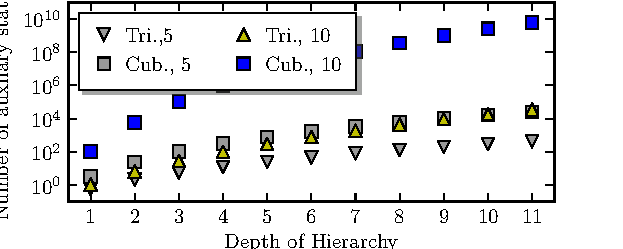
\includegraphics{img/scaling.pdf}
  \caption{%
    Scaling of the number of auxiliary states with the truncation order $D$ and number of modes $N$.
    Even for relatively small $N$ the triangular scheme~\ref{eq:num.triangular_scaling} is far superior compared to the cubic truncation scheme with an exponential scaling law $(D+1)^N$.
  }
  \label{fig:num.scaling}
\end{figure}
%%%%%%%%%%%%%%%%%%%%%%%%%%%%%%%%%%%%%%%%%%%%%%%%%%%%%%%%%%%%%%%%%%%%%%%%%%%%%%%%

Examining \autoref{eq:num.hierarchy_lin_multi} closer we notice that the term responsible for suppression of the $\kk$\th auxiliary state is $\exp(-\kk \cdot \ww)$.
Instead of treating each mode individually we use a condition better suited for the product $\kk\cdot\ww$, namely $0 \le \abs{\kk} \le D$ with $\abs{\kk} = \sum_j k_j$.
% FIXME Use truncation picture?
%For $N=2$ the corresponding states form a triangular shape as shown in \autoref{fig:num.trunc_tria}---hence the name \quotes{triangular truncation scheme}.
For $N=2$ the corresponding states form a triangular shape---hence the name \quotes{triangular truncation scheme}.
The appropriate generalization to an arbitrary number of modes is a $N$-simplex with the number of elements given by
\begin{equation}
  \sum_{d=0}^D {d + N - 1 \choose N - 1} = \frac{(D + N)!}{D!N!},
  \label{eq:num.triangular_scaling}
\end{equation}
showing a much softer scaling with $N$ compared to the cubic scheme.
In \autoref{fig:num.scaling} we display the number of auxiliary states required for a given number of modes and truncation order $D$:
Clearly the triangular truncation is far superior although for small $N$ both methods are applicable.
The difference is more pronounced for larger $N$ required in the study of realistic systems.
% FIXME What was really done?
As an example take the Fenna-Matthews-Olson complex further investigated in \autoref{sec:num.fmo}:
In a simplified model we couple mutually independent environments with 13 exponential terms to each of its seven sites for a total of 91 modes.
This yields an insurmountable number of about $10^{30}$ auxiliary states for the cubic truncation in first order hierarchy, compared to only 5151 using the triangular scheme.

Depending on the specific problem, additional truncation conditions may reduce the computational expenses without sacrificing accuracy.
Especially environments mixing modes with large memory times and almost-Markovian modes provide many options for optimization.
However, we do not elaborate this point any further and rely on the triangular truncation throughout this work.

%%%%%%%%%%%%%%%%%%%%%%%%%%%%%%%%%%%%%%%%%%%%%%%%%%%%%%%%%%%%%%%%%%%%%%%%%%%%%%%
\section{Correlation Function Expansion}
\label{sec:num.expansion}
% * pade spectrum decomposition
% * also mention other (Matsubara e.g.)
% * uniqueness? Theoretically yes, in practices doesnt matter!
% * Plot for Ohmic spectral density (where do these appear?)
% * Show highly structured density, approximation!
%
% TODO Expansion of general spectral density; not unique!
%      Cool to use antisymmetric lorentzians

%%%%%%%%%%%%%%%%%%%%%%%%%%%%%%%%%%%%%%%%%%%%%%%%%%%%%%%%%%%%%%%%%%%%%%%%%%%%%%%

Applicability of our hierarchical equations of motion to certain model depends predominantly on the ability to express the relevant bath correlation function
\begin{equation}
  \alpha(t-s) = \int_0^\infty J(\omega) \left( \coth \frac{\beta \omega}{2} \cos \omega(t-s) - \ii\sin \omega(t-s) \right) \mathrm{d}\omega
  \label{eq:num.alpha_thermal}
\end{equation}
as a sum of exponentials like~\ref{eq:num.exp_bcf}.
Such exponentials arise as Fourier transforms of a Lorentzian spectral density
\begin{equation}
  J(\omega) = \frac{1}{\pi} \frac{\gamma}{(\omega - \Omega)^2 + \gamma^2}.
  \label{eq:num.lorentzian}
\end{equation}
Hence they can be obtained from \autoref{eq:num.alpha_thermal} in the zero-temperature limit provided we extend the integral domain to include arbitrary negative frequencies as well.
This unphysical assumption seems to be a good approximation to the exact case without negative frequencies for certain parameters as \autoref{fig:num.lorentzian} shows:
For $\gamma\ll\Omega$ the Lorentzian density $J$ is concentrated on the positive semi-axis and the negative frequency contributions vanish primarily.
However, \autoref{eq:num.lorentzian} is a prime example of a heavy-tailed distribution, having no finite moments except $\int J(\omega) \dd \omega = 1$---thus making such a hand-waving statement questionable.\\

%% Lorentzians %%%%%%%%%%%%%%%%%%%%%%%%%%%%%%%%%%%%%%%%%%%%%%%%%%%%%%%%%%%%%%%%%
\begin{figure}
  % TODO Same parameters, but antisymmetrized
  \centering
  \includegraphics{img/lorentzian}
  \caption{%
    Schematic comparison of Lorentzian spectral densities used to obtain exponential bath correlation functions (see \autoref{eq:num.lorentzian} for notation).
    For $\gamma\ll\Omega$ (blue line) the weight is concentrated on the positive semi-axis.
  }
  \label{fig:num.lorentzian}
\end{figure}
%%%%%%%%%%%%%%%%%%%%%%%%%%%%%%%%%%%%%%%%%%%%%%%%%%%%%%%%%%%%%%%%%%%%%%%%%%%%%%%%

A more systematic way to obtain the desired bath correlation function in the case $T > 0$ involves anti-symmetrized spectral densities $\tilde J(\omega) := J(\omega) - J(-\omega)$
This way negative frequencies are included without any approximation.
Indeed, since $\tilde J$, $\coth$, and $\sin$ are anti-symmetric and $\cos$ is symmetric with respect to reflection at the origin we have
\begin{equation}
  \int_0^\infty \tilde J(\omega) (\dots) \mathrm{d}\omega = \frac{1}{2}\int_{-\infty}^\infty \tilde J(\omega) (\dots) \mathrm{d}\omega.
  \label{eq:num.correlation_integral}
\end{equation}
% FIXME Citation for Drude
Commonly used examples are Drude spectral densities in the \HEOM-formalism \cite{} or anti-symmetrized Lorentzians, which are well suited to approximate highly-structured environments \cite{MeTa99_non_markovian}.
Although the discussion below works a much larger class of spectral densities \cite{RiEi13_bcf}, we assume $\tilde J$ with a finite number of mutually distinct poles lying off the real and imaginary axis---like $\tilde J$ obtained from \autoref{eq:num.lorentzian}.

To calculate the correlation function, we evaluate the integral~\ref{eq:num.correlation_integral} analytically using the residue theorem.
While the poles of the anti-symmetric spectral density $\tilde J$ are assumed to be known, there are two different expansion schemes for the hyperbolic cotangens:
% FIXME in in
Since many established \HEOM-results are based on the Matsubara-spectrum decomposition, it is presented in detail first.
Nevertheless, it has been brought forward only recently that the Padé-expansion provides superior convergence in terms of the number of poles.
As the latter is crucial for numerical efficiency, \autoref{sub:num.expansion.pade} contains some remarks on the latter.
In what follows we focus on the real part of \autoref{eq:num.correlation_integral} given by
\begin{equation}
  a(t) = \frac{1}{2} \int_{-\infty}^\infty \tilde J(\omega) \coth \frac{\beta\omega}{2} \cos \omega t \dd\omega
  = \frac{1}{2} \int_{-\infty}^\infty \tilde J(\omega) \coth \frac{\beta\omega}{2} \exp[\ii \omega t] \dd\omega,
  \label{eq:num.alpha_thermal_re}
\end{equation}
since it encodes all thermal effects.
Calculating the corresponding imaginary part is straightforward.


%%%%%%%%%%%%%%%%%%%%%%%%%%%%%%%%%%%%%%%%%%%%%%%%%%%%%%%%%%%%%%%%%%%%%%%%%%%%%%%
\subsection{Matsubara Spectrum Decomposition}
\label{sub:num.expansion.matsubara}

A commonly used expansion scheme for the hyperbolic cotangens is the Matsubara spectrum decomposition \cite{Ma00_many_particle}
\begin{equation}
  \coth\left(\frac{\beta \omega}{2}\right) = \frac{2}{\beta} \sum_{n=-\infty}^\infty \frac{1}{\ii\xi_n - \omega},
  \label{eq:num.matsubara_expansion}
\end{equation}
with the Matsubara frequencies $\xi_n = 2\pi n / \beta$.
A short proof and remarks on the convergence of the series above is given in \autoref{sec:coth.matsubara}.
Clearly, all poles of the $\coth$ lie on the imaginary axis and are therefore distinct from those of the spectral density by assumption.
This allows us to express \autoref{eq:num.alpha_thermal_re} as a sum-over-poles with non-negative imaginary parts, after closing the integration contour in the upper complex half-plane for $t > 0$:
\begin{equation}
  a(t) = \sum_{\omega'} \Res_{\omega'}(\tilde J) \, \coth \frac{\beta \omega'}{2} \exp[\ii\omega' t]
  + \sum_{\xi_n > 0} \Res_{\ii\omega_n} \left(\coth \frac{\beta\cdot}{2} \right) \, \tilde J(\ii\xi_n) \exp[-\xi_n t].
  \label{eq:num.sum_over_poles}
\end{equation}
Here the first sum involves all poles $\omega'$ of $\tilde J$ with $\Im \omega' > 0$.
No special care is needed for the coth-pole at $\omega = 0$ since $\tilde J(0)$ vanishes anyway.
Clearly, $a(t)$ has the desired exponential form.

As $\exp[-\xi_n t]$ suppresses contributions from large Matsubara frequencies unless $t$ is very small, the infinite sum in \autoref{eq:num.sum_over_poles} is truncated at finite order for numerical purposes.
The calculation for $t < 0$ and the imaginary part of \autoref{eq:num.alpha_thermal} runs along the same lines.


%%%%%%%%%%%%%%%%%%%%%%%%%%%%%%%%%%%%%%%%%%%%%%%%%%%%%%%%%%%%%%%%%%%%%%%%%%%%%%%
\subsection{Padé Spectrum Decomposition}
\label{sub:num.expansion.pade}
%
% TODO Comparisson of both

Although the Matsubara $\coth$-expansion provides the sought-after exponential decomposition of the bath correlation function, it is worthwhile to consider alternative schemes---especially since the computational effort of our hierarchical equations of motion depends crucially on the numbers of modes under consideration.
Only recently Hu et al.\ proposed an expansion based on the Padé approximant \cite{HuXuYa10_pade,Hu11_pade}, which is vastly superior to the Matsubara-approach in terms of convergence speed.
For further details on the theory of Padé approximants see the book by Baker and Graves-Morris \cite{BaGr96_pade}, here we only provide the basic ideas necessary for our exponential-representation.

To start off we recall that the hyperbolic cotangens has a simple pole at $z=0$ with $\Res_0(\coth) = 1$; therefore we have the convergent Taylor series
\begin{equation}
  f(z) := \coth z - \frac{1}{z} = \lim_{N\to\infty} z \sum_{k=0}^{2N-1} a_k z^{2k} = \lim_{N\to\infty} z \, f_{2N-1}(z^2)
  \label{eq:num.coth_expansion},
\end{equation}
where we use that $\coth$ as well as $z \mapsto 1/z$ are anti-symmetric functions, causes all even terms in the Taylor series to vanish.
Below we employ the abbreviation $x = z^2$.
By definition of the coefficients $a_k$ we have $f(z) - z \, f_{2N-1}(z^2) = \mathcal{O}(z^{4N + 1})$ for $\abs{z} < \pi$.
In fact the radius of convergence cannot be increased any further since there are additional singularities of the hyperbolic cotangens at $z = \pm\ii\pi$ and the approximating functions $f_N$ are analytical.

Using a Padé approximant basically amounts to incorporating these poles into the approximating functions.
The simplest choice is the class of rational functions, that is functions of the form $f_{M,N}(x) = P_M(x) / Q_N(x)$ with polynomials $P_M$ and $Q_N$ of degree less than $M$ and $N$ respectively.
We refer to these as $[M,N]$-approximants.
For the sake of simplicity, we only consider approximants of class $[N-1, N]$, which have proven especially suitable for Bose-Einstein and Fermi-Dirac distribution functions \cite{Hu11_pade}.

In order to replace $f_N$ in \autoref{eq:num.coth_expansion} by a $[N-1,N]$ Padé approximant $f_{N-1,N}$, the latter needs to fulfill the interpolation condition
\begin{equation}
  f_{2N-1}(x) = \sum_k^{2N-1} a_k x^k = \frac{P_{N-1}(x)}{Q_N(x)} + \mathcal{O}(x^{2N}).
  \label{eq:num.pade_interpolation}
\end{equation}
In other words, $f_{N-1,N}$ is the rational function of degree $N-1$ and $N$, respectively, that coincides with the Taylor-series of $f$ around $x = 0$ up to $x^{2N}$.
Unless $Q_N(0) = 0$ this is equivalent to $Q_N(x)f_{2N-1}(x) = P_{N-1}(x) + \mathcal{O}(x^{2N})$, which always has a unique solution as shown by comparing coefficients on both sides.
Using the Padé approximant, we can rewrite \autoref{eq:num.coth_expansion} as
\begin{equation}
  \coth(z) = \frac{1}{z} + \frac{z P_{N-1}(z^2)}{Q_N(z^2)} + \mathcal{O}(z^{4N+1})
  \label{eq:num.coth_pade}
\end{equation}
Although $P_{N-1}$ and $Q_N$ are of degree $N-1$ and $N$, respectively, there are only $2N$ free parameters because both are fixed only up to a common prefactor.
Therefore $f_{N-1,N}$ and $f_{2N-1}$ have the same number of coefficients to be determined.\\



Remarkably, the Padé approximant not only converges on larger subset of $\Complex$ than the power series in general, but also provides a superior sum-over-poles decomposition for a finite number of terms compared to the Matsubara expansion~\ref{eq:num.matsubara_expansion}.
It turns out that the roots of $Q_N$ are mutually distinct and negative \cite{HuXuYa10_pade}; therefore we denote them by $\xi_i^2$ ($i=1,\dots,N$).
Therefore the truncated pole-decomposition of the hyperbolic cotangens can be written as
\begin{equation}
  \coth\left( \frac{\beta\omega}{2} \right) = \frac{2}{\beta\omega} + \frac{2}{\beta} \sum_{j=1}^N \left( \frac{\eta_j}{\omega + \ii\xi_j} + \frac{\eta_j}{\omega - \ii\xi_j} \right) + \mathcal{O}(\omega^{4N+1})
  \label{eq:num.pade_expansion}
\end{equation}
which agrees with \autoref{eq:num.matsubara_expansion} for $N\to\infty$.
It is only for a finite number of summands that the Padé expansion comes to fruition.
As an example take $N=5$, then we find
\begin{align*}
  \left( \frac{\beta \xi_j}{2\pi j} \right)_j &= (1.00, 1.00, 1.01, 1.18, 2.69) \\
  \left( \frac{\beta\eta_j}{2} \right)_j &= (1.00, 1.00, 1.11, 2.80, 26.59),
\end{align*}
showing a noticeable different behavior than the Matsubara poles and residues, namely $\beta \xi_j/2\pi j = 1$ and $\beta \eta_j/2 = 1$.
Because in the calculation of the bath correlation function~\ref{eq:num.sum_over_poles} the suppressing term is given by $\exp^{-\xi_j t}$, the super-linear growth of the Padé poles ensure a much higher accuracy for a small number of modes.
% TODO Ref or picture to compare
% TODO Downsides

In conclusion the Padé spectrum decomposition~\ref{eq:num.pade_expansion} can be interpreted as an optimally-corrected finite Matsubara expansion, where neglected terms are included by adjusting the final poles and residues.


%%%%%%%%%%%%%%%%%%%%%%%%%%%%%%%%%%%%%%%%%%%%%%%%%%%%%%%%%%%%%%%%%%%%%%%%%%%%%%%
\section{Spin-Boson Model}
\label{sec:num.spin_boson}
% * short intro
% * Depth-dependence
% * Terminator dependence
% * lin vs nonlin ✔
% * nr. of realizations for different sets of paramters ✔
% * single trajectories ✔
% * divergences for large coupling --> cause bad truncation
%
% TODO Add application citations
% TODO Better convergence criterion than "looks good"
% TODO What about γ=0 convergence? Sample Size?
% TODO ASKWALTER: How many details on numerical parameters
%%%%%%%%%%%%%%%%%%%%%%%%%%%%%%%%%%%%%%%%%%%%%%%%%%%%%%%%%%%%%%%%%%%%%%%%%%%%%%%


The Spin-Boson model is a paradigmatic system used in the theoretical description of dissipative quantum dynamics \cite{Le87_spinboson,We99_dissipative_systems}.
Despite being comparatively simple and numerically tractable, it displays properties also found in more complex systems---take for example the transition between a localized, essentially classical phase and a delocalized phase allowing quantum mechanical tunneling \cite{FlVeNa10_spin_boson}.
Therefore it is well suited to investigate properties of dissipative system and the influence of an environment in general.
Furthermore, it is often employed as an approximate description of systems with a continuous degree of freedom confined by a double well potential.
Examples for the latter are the motion of defects in some crystalline solids or magnetic flux trapped in a superconducting qubit \cite{CaLe83_diss_system}.
We use it to demonstrate the superiority of the nonlinear compared to the linear hierarchy as well as the convergence of our hierarchy with increasing depth.

The Spin-Boson model consists of a two-level system with the free time evolution described by the Hamiltonian
\begin{equation*}
  \Hsys = - \frac{1}{2}\Delta \sigma_x + \frac{1}{2} \epsilon \sigma_z,
\end{equation*}
coupled linearly to a bath of harmonic oscillators with $L=\sigma_z$.
For simplicity, all calculations in this section involve only a single exponential bath mode with correlation function $\alpha(t) = g \,\exp[-\gamma \abs{t} - \ii\Omega t]$.


%%%%%%%%%%%%%%%%%%%%%%%%%%%%%%%%%%%%%%%%%%%%%%%%%%%%%%%%%%%%%%%%%%%%%%%%%%%%%%%%
\subsection{Sample Size}
\label{sub:num.spin_boson.sample_size}
%
% TODO Perturbative calculation?
% TODO What about γ

\begin{figure}[p]
  \centering
  \includegraphics{img/linvsnonlin_averaged.pdf}
  % TODO Add parameters
  \caption{%
    Expectation values for the $\sigma_z$-operator calculated using the linear (left) and nonlinear (right) hierarchical equations for two sets of parameters.
    On the top we display a weakly coupled system given by parameters\dots
    In contrast the bottom pictures show a strongly coupled system with\dots
  }
  \label{fig:num.linvsnonlin}
\end{figure}

% FIXME of of of
Since our hierarchy is based upon a stochastic differential equation, it is crucial to assess its reliability in dependence on the sample size.
In this section we study the convergence of our Monte-Carlo average with respect to the number of realizations.
We emphasize in particular the superiority of the nonlinear version~\ref{eq:num.hierarchy_nonlin} over the linear hierarchy~\ref{eq:num.hierarchy_lin}.
To really emphasize the strengths and weaknesses of both approaches, we choose two quite distinct sets of parameters.
Although it is not the only difference between both sets, we refer to them as the weakly and strongly coupled parameters.
The former can even be treated using an improved perturbation scheme \cite{GaHuZh10_qubit,HuZh08_qubit}.

In \autoref{fig:num.linvsnonlin} we plot the expectation value of the spin-operator in $z$-direction for an initial eigenstate \quotes{spin up}.
In the case of weak coupling, shown at the top, there seems to be almost no difference between the linear version on the left and the nonlinear version on the right.
Nevertheless for very few realizations the latter is still in better agreement with the more accurate results.
Especially for large times the dampening on the right hand side is more pronounced as comparing the graph for a sample size of ten reveals.

When it comes to the strongly coupled parameter set at the bottom, the picture changes dramatically:
First notice that the sample size has been increased by an order of magnitude to obtain a reliable result.
Notwithstanding the linear version does not display any visible changes for the different sample sizes shown; hence we cannot expect convergence for even larger numbers of realizations.
It is only for very small times that both, left and right picture, agree up to a certain extent.
In contrast, the nonlinear version improves steadily with growing sample size and already provides a very good approximation with only minor fluctuations at 1000 trajectories.
Remarkably, even 100 realizations produce the correct qualitative features as the vanishing of $\qmean{\sigma_z}$ for large $t$---the linear hierarchy is not capable of producing equally good results using a sample size more than 100 times larger.\\

\begin{figure}[t]
  \centering
  \includegraphics{img/normcomp.pdf}
  % FIXME Caption
  \caption{%
    Contributions of single trajectories to the reduced density operator for the linear equations.
    Left: weakly; right: strongly
    For definition see \autoref{eq:num.contribution}\dots
    Parameters are the same as in \autoref{fig:num.linvsnonlin}
    Dotted line = nonlinear.
  }
  \label{fig:num.normcomp}
\end{figure}

To understand this behavior, recall that we have introduced the nonlinear equations in order to achieve an average over single realizations contributing equal amounts.
As already mentioned in \autoref{sec:nmqsd.nonlin_nmsse}, individual trajectories of the linear version violate this requirement more or less severely.
In order to get a better assessment of different contributions over time we have to rescale the norm as follows:
First we calculate the reduced density operator $\rho_t$ by the usual Monte-Carlo average
\begin{equation}
  \rho_t = \sum_{n=1}^N \ket{\psi_t(\ZZ_n)} \bra{\psi_t(\ZZ_n)}
  \label{eq:num.monte_carlo_avg}
\end{equation}
over a large number of noise process realizations $\ZZ_n$.
Afterwards we obtain a genuine, normalized density matrix by rescaling with $(\Tr{} \rho_t)^{-1}$.
Therefore we can assess the contribution of a single trajectory $\psi_t(\ZZ_n)$ to \autoref{eq:num.monte_carlo_avg} by $\lfloor \psi_t(\ZZ_n) \rfloor / N$ with
\begin{equation}
  \lfloor \psi_t(\ZZ_n) \rfloor = \sqrt{%
    \frac{\sp{\psi_t(\ZZ_n)}{\psi_t(\ZZ_n)}}{\Tr{} \rho_t}.
  }
  \label{eq:num.contribution}
\end{equation}
Since for the nonlinear equation the average in \autoref{eq:num.monte_carlo_avg} is taken over normalized states $\tilde\psi(\ZZ_n) = \psi(\ZZ_n) / \abs{\psi(\ZZ_n)}$, the corresponding contribution $\lfloor \tilde\psi_t(\ZZ_n) \rfloor / N$ is one.

\Autoref{eq:num.normcomp} shows the contribution of a few single realizations used on the left hand side of \autoref{fig:num.linvsnonlin}; clearly we obtain quite different results for both parameter sets.
But for the weakly coupled system on the left all trajectories remain roughly in the same order of magnitude.
In contrast, the contributions on the right hand side, belonging to the strongly coupled system, all vanish for large $t$, but also show pronounced peaks for a few trajectories.

% TODO Does gamma have any influence???
We conclude, that the nonlinear hierarchy is a drastic improvement in terms of numerical efficiency for the strongly coupled system, since the additional complexity is more than compensated by the reduced sample size.
Beside the coupling strength, the major difference between both parameter sets is the much smaller $\gamma$ of the weakly coupled system\dots

Therefore all subsequent calculations shown in this work are based on the nonlinear hierarchy unless stated otherwise.


%%%%%%%%%%%%%%%%%%%%%%%%%%%%%%%%%%%%%%%%%%%%%%%%%%%%%%%%%%%%%%%%%%%%%%%%%%%%%%%%
\subsection{Hierarchy Depth and Cutoff}
\label{sub:num.spin_boson.depth}
%
% TODO Cutoff criterion sqrt...

Apart from the sample size there is an even more significant factor limiting the applicability of our hierarchical equations of motion:
As seen from \autoref{fig:num.scaling} the number of auxiliary states required---and with it the computational expense---grows faster then linear with the truncation depth.
Before investigating the latter more thoroughly we demonstrate the effectiveness of using an appropriate terminator instead of just truncating the hierarchy.
For that matter the Spin-Boson model is well suited since contrary to the Dissipative two-level system presented in \autoref{sec:nmqsd.two_level} it does not terminate at any finite order.
